% easychair.tex,v 3.5 2017/03/15

\documentclass{easychair}
%\documentclass[EPiC]{easychair}
%\documentclass[EPiCempty]{easychair}
%\documentclass[debug]{easychair}
%\documentclass[verbose]{easychair}
%\documentclass[notimes]{easychair}
%\documentclass[withtimes]{easychair}
%\documentclass[a4paper]{easychair}
%\documentclass[letterpaper]{easychair}

\usepackage{cleveref}
\usepackage{doc}
\usepackage{tabularx}
% use this if you have a long article and want to create an index
% \usepackage{makeidx}

\lstset{
  frame=none,
  xleftmargin=2pt,
  stepnumber=1,
  numbers=left,
  numbersep=5pt,
  numberstyle=\ttfamily\tiny\color[gray]{0.3},
  belowcaptionskip=\bigskipamount,
  escapeinside={*'}{'*},
  tabsize=2,
  emphstyle={\bf},
  commentstyle=\color{ForestGreen},
  stringstyle=\mdseries\rmfamily,
  showspaces=false,
  keywordstyle=\bfseries\rmfamily,
  columns=flexible,
  basicstyle=\small\sffamily,
  showstringspaces=false,
  morecomment=[l]\%,
}

\lstset{basicstyle=\footnotesize\ttfamily,breaklines=true}
% In order to save space or manage large tables or figures in a
% landcape-like text, you can use the rotating and pdflscape
% packages. Uncomment the desired from the below.
%
% \usepackage{rotating}
% \usepackage{pdflscape}

% Some of our commands for this guide.
%
\authorrunning{Lukas Abelt}


\newcommand{\LayeredTypes}{\textsc{LayeredTypes}}
\newcommand{\Lark}{\textsc{Lark}}
%\makeindex

\makeatletter
\def\input@path{{../chapters}}
%or: \def\input@path{{/path/to/folder/}{/path/to/other/folder/}}
\makeatother
\graphicspath{{../graph}}



%% Front Matter
%%
% Regular title as in the article class.
%
\title{Industry Internship -- Final Report}

% Authors are joined by \and. Their affiliations are given by \inst, which indexes
% into the list defined using \institute
%
\author{
Lukas Abelt\inst{1,2}
}

% Institutes for affiliations are also joined by \and,
\institute{
   Saarland University,
   Germany\\
   \email{luab00001@stud.uni-saarland.de}
  \and
   LASIGE,
  Faculdade de Ciências da Universidade de Lisboa, Portugal\\
  \email{labelt@lasige.di.fc.ul.pt},
}



\titlerunning{Industrial Internship Report}


\begin{document}
\maketitle

%------------------------------------------------------------------------------
\section{About this document}

This document composes the internship report for the industrial internship of Lukas Abelt, carried out from October 2022 until March 2023 at the LASIGE Research Centre in Lisbon, Portugal. 

\section{Internship Overview}
This seciton gives an overview of the relevant key data of persons and institutions involved in this internship.

\begin{tabularx}{\textwidth}{rX}
	\textbf{Name of Intern/Student:} & Lukas Abelt\\
	\textbf{Student Contact Information:} & \email{luab00001@stud.uni-saarland.de}\\
	\textbf{Matriculation Number at UdS:} & 7009048\\
	\textbf{Course of Study at UdS:} & Master of Science Computer Science\\
	\textbf{Start of Internship:} & 01.01.2022\\
	\textbf{End of Internship:} & 31.03.2023\\
	\textbf{Hosting Insitution:} & LASIGE Research Unit\footnote{\url{https://www.lasige.pt/}}\newline Reliable Software Systems Research Line\newline Faculdade de Ciências da Universidade de Lisboa\\
	\textbf{Internship Supervisor:} & Alcides Fonseca, Assistant Professor\\
	\textbf{Supervisor Contact Information:} & \email{amfonseca@fc.ul.pt}\\
	\textbf{Internship Title:} & \textit{Type Layers for Gradual Verification}
\end{tabularx}

\section{Internship Description}
This section will give a bread overview of the work that was carried out during the internship. It wstart by providing context to the problem at hand and continue further with the proposed approach and goals of the internship. A technical description of the implemented solution will be provided and finally a short overview of the acquired skills and produced deliverables will be provided.

\subsection{Context}
\label{sec:context}
Most programmers and computer scientists will be familiar with simple type systems that ensure that the code they write is type safe in the context of the language they are writing it in. However, much more sophisticated type systems exist that can be used to ensure specific properties of a program, such as resource usage (Linear Types~\cite{linear}), value predicates (Liquid Types~\cite{DBLP:conf/pldi/RondonKJ08}), or correct following of a distributed protocol (Session Types~\cite{session}).

Some of these type systems can be dependent or independent from each other. Both Liquid Types and Session Types require a base type system with primitive types (such as int, bool) to exist, but they can be orthogonal to each other, as you can have a Liquid Type whose base type is int, and a Session Type that also relies on the base value being int, ignore the liquid predicate.

Given this plethora of type systems, different applications require a different subset of type systems. Not all applications require these advanced type systems (e.g., fully dependent types), trading off static guarantees for (even if short-term) productivity. Untyped languages have been popular in both web applications, scripting and data science. On the other hand, if you are writing a device driver, you will probably want to take advantage of a type system that guarantees that memory usage is constrained to a given bound~\cite{liquidate-assets}. Or if you are writing a complex, distributed protocol, you might want to take advantage of Session Types for that part of the program.

During this internship, we tried to address the challenge of how can multiple type system co-exist in the same programming language, allowing different, valid combinations to be used in the type-checking of a program.
 
 To illustrate this in a small example, consider the program in \Cref{lst:code_before} that reads the text contents of a file and prints it to the console line-by-line. In this short snippet, there are multiple concerns to be addressed. Firstly, one wants to ensure that all function calls are done with variables of the appropriate data types. Secondly, to avoid errors due to an out of bound access, \texttt{get} should only be called with an index that does not exceed the list length. Lastly, when working with resources such as a file descriptor it might be useful to track it's state and ensure that it is in a proper (closed) state at the end of program execution. Note that the same standard library functions (\lstinline|createFD|, \lstinline|readLines|, etc...) may be needed in other programs with different type systems requirements.

These properties can be verified in two major ways. 

All features from all type systems can be combined in single, monolithic type system, containing all the complexity that all the different type systems entail. A very similar issue can also be observed when operating on Liquid Types: In certain cases we want to define predicates on orthogonal properties that could be verified independently from one another; However, current implementation of liquid types do not allow such distinction, leading to confusing and unintelligible error messages~\cite{wits-error-messages}. 

\subsection{Goals}
\label{sec:proposed-approach}
The Goals of the internship was to explore a new verification approach, which was later decided to be called \LayeredTypes. In \LayeredTypes, developers can write programs, but can also define additional type systems as layers. Each layer defines the basic types, and how typechecking happens. Additionally, a layer may depend on another layer if it requires information (such as types or typing contexts) from another layer.

Type checking of programs can be partial in the sense that a program may only use some layers (even if the libraries used are defined in more layers), requiring only that each function contains type information for that layer and all dependencies. The missing layers can be added over time, if they are found to be relevant.

For this purpose, a prototype was to be developed consisting of a small and simple functional language accompanied by a prototype layered Verification tool that can realise the described layered verification approach.

We believe that this layered, incremental approach can help build more powerful and independent type systems while at the same time making it simpler to understand the errors that might arise during verification.

\subsection{Implementation Details}

We developed a prototype for a layered verification approach called \LayeredTypes. In this prototype, programs can be written in a simple functional language that supports some primitive operations such as variables, function definitions, basic binary operations and \texttt{let} constructs. To enable the use of more complex functionality, it is also possible to define additional functions in python that can be called in this simple language. An example of a program written in that language can be seen in \Cref{lst:code_before}.

The prototype consists of a simple compiler and interpreter for said functional language. The prototype has been developed in Python using the \Lark compiler framework. The core of our compiler is a \textit{layered static verifier}. Within a program, the programer can define annotations to be passed on to one or multiple verification layers. The implementation of each verification layer is provided by the programer in a separate python file with a pre-defined set of functions that will be called by the verifier. Specifically, each layer can provide the following information:

\begin{itemize}
	\item A list of all other layers that it depends on -- That is, all layers that need to be verified successfully before the layer itself is verified
	\item A list of all layers that should be run \textit{after} this layer has been successfully verified
	\item A \texttt{typecheck} function that gets passed the AST of the program and can perform the specific verification for the current layer.
\end{itemize}

The framework will build the dependency graph of all layers defined and used in a program and run them in a topological order so that all dependencies are satisfied. A conceptual overview of the verification framework can be seen in \Cref{fig:framework_overview}

\begin{figure}[ht!]
	\centering
	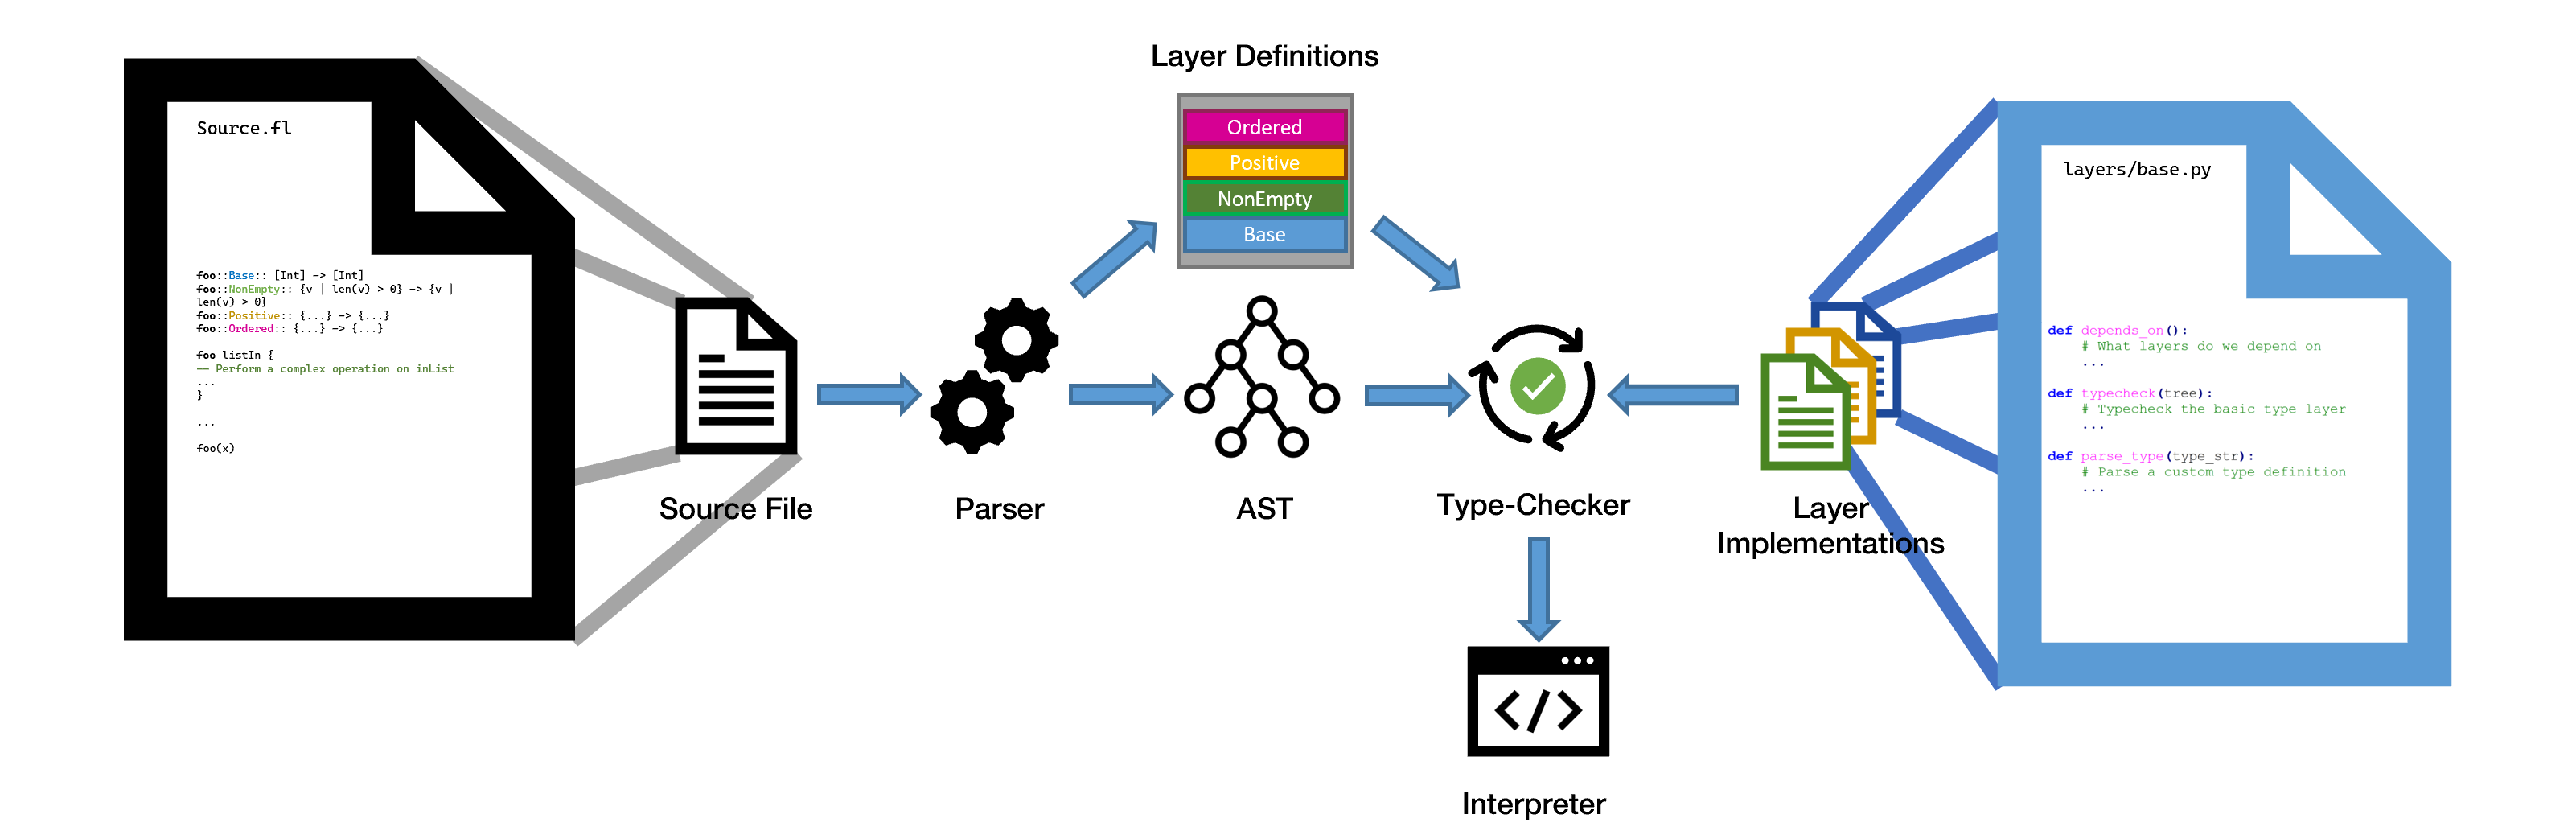
\includegraphics[width=.8\textwidth]{framework_overview}
	\label{fig:framework_overview}
	\caption{Conceptual Overview of \LayeredTypes}
\end{figure}

To evaluate our work, we also implemented two different use-cases:

In the first Use-Case, we developed a simple program that reads input from a file and processes it line by line. In this use-case we use three different layers. The first layer, \texttt{types} is a simple layer that is used to annotate typing information to variables and functions. The second layer, \texttt{typecheck}, depends on the first one and defines rules on how the program should be type-checked. It then uses the annotations provided by the \texttt{type} layer to check if the program is well-typed. The third layer, \texttt{state}, can be used to define, check and transistion states on variables. In our example we use it to track the state of the file descriptor and ensure that it is closed at the end of the program. The \texttt{state} layer acts independently from the other two layers.

In the second Use-Case we focus on a problem currently present in implementations for \textit{Liquid Types}:

\subsection{Deliverables and Publications}

The full implementation of the developed prototype of \LayeredTypes will be published on GitHub\footnote{\url{https://github.com/LuAbelt/LayeredTypes}}. In addition a submission for a contributed talk was made to the TYPES2023 conference\footnote{\url{https://types2023.webs.upv.es/Index.html}} that is still pending a notification of acceptance or rejection. Additionally it is planned to potentially submit a paper to a relevant conference later in 2023.

\section{Acknowledgments}
\label{sec:acknowledgments}
This work was supported by \textit{Fundação para a Ciência e Tecnologia} (FCT) in the LASIGE Research Unit under the ref. UIDB/00408/2020 and UIDP/00408/2020, by the CMU--Portugal project CAMELOT (LISBOA-01-0247-FEDER-045915), and the RAP project under the reference (EXPL/CCI-COM/1306/2021).


\bibliographystyle{plain}
\bibliography{literature.bib}
\begin{minipage}{0.4\linewidth}
\begin{lstlisting}[caption={Simple example code},label={lst:code_before}]
printLines lines idx len {
  if len != idx then {
    line = get(lines, idx)
    print(line)
    printLines(lines, idx+1, len)
  }
}

filename = "input.txt"
fileDescriptor = createFD(filename)

open(fileDescriptor)

lines = readLines(fileDescriptor)
len = length(lines)
printLines(lines, 0, len)

close(fileDescriptor)
\end{lstlisting}
\end{minipage}%
\begin{minipage}{0.59\linewidth}
\begin{lstlisting}[caption={Annotations for \LayeredTypes},label={lst:code_after}]
-- State Layer definitions
createFD :: state :: {} -> { Closed }
openFile :: state :: {Closed => Open} -> {}
readLines :: state :: {Open => Consumed} -> {}
closeFile :: state :: {Consumed => Closed} -> {}

-- Type layer definitions
get :: types :: List -> int -> string
length :: types :: List -> int
createFD :: types :: string -> FileHandle
open :: types :: FileHandle -> void
readLines :: types :: FileHandle -> List
close :: types :: FileHandle -> void
print :: types :: string -> void
printLines :: types :: List -> int -> int -> void

-- Liquid layer definitions
length :: {List | true} -> {v:int | v>=0}
printLines :: liquid :: { List | true } -> { l:int | l>=0 } -> { i:int | i<=l }
get :: liquid :: { List | true } -> { i:int | i<len }

-- State requirement at the end of the program
fileDescriptor :: state :: {Closed}	
\end{lstlisting}
\end{minipage}


\end{document}

%------------------------------------------------------------------------------
